\documentclass{beamer}
\usepackage[russian]{babel}
\usetheme{metropolis}

\usepackage{amsthm}
\setbeamertemplate{theorems}[numbered]

\setbeamercolor{block title}{use=structure,fg=white,bg=gray!75!black}
\setbeamercolor{block body}{use=structure,fg=black,bg=gray!20!white}

\usepackage[T2A]{fontenc}
\usepackage[utf8]{inputenc}

\usepackage{hyphenat}
\usepackage{amsmath}
\usepackage{graphicx}

\AtBeginEnvironment{proof}{\renewcommand{\qedsymbol}{}}{}{}

\title{
Микроэкономика-I
}
\author{
Павел Андреянов, PhD
}

\begin{document}
\maketitle

\section{Рынок одного товара}

\begin{frame}{Рынок одного товара}
	
В этой лекции мы поговорим о собственно кривых спроса и предложения, которые получаются в результате решения задач потребителя и производителя. Потребитель создает кривые спроса на конечные товары, а производитель на факторы. Также, производитель создает кривые предложения.

Важным моментом во всем последующем анализе является то, что мы фокусируемся на рынке одного единственного товара, на который есть спрос и предложение. Это называется \textbf{частичным равновесием}. Остальные товары, спросы и цены на них, выносятся за рамки анализа.

Пусть количество интересующего нас товара, а также равновесная цена на него обозначаются $Q,P$.
	
\end{frame}

\section{Сдвиги кривых спроса (на товары)}

\section{Появление субститутов}

\begin{frame}{Появление субститутов}
Зафиксируем кривую предложения $Q^s(P)$.

Когда появляется новый субститут на товар, то мы считаем, что спрос на него падает (сокращается). На самом деле, не просто спрос в равновесии, а вся кривая спроса $Q^d(P)$ падает, в том смысле, что при одной и той же цене, потребители согласны купить меньше этого товара.

\end{frame}

\begin{frame}{Появление субститутов}
\begin{figure}[hbt]
\centering
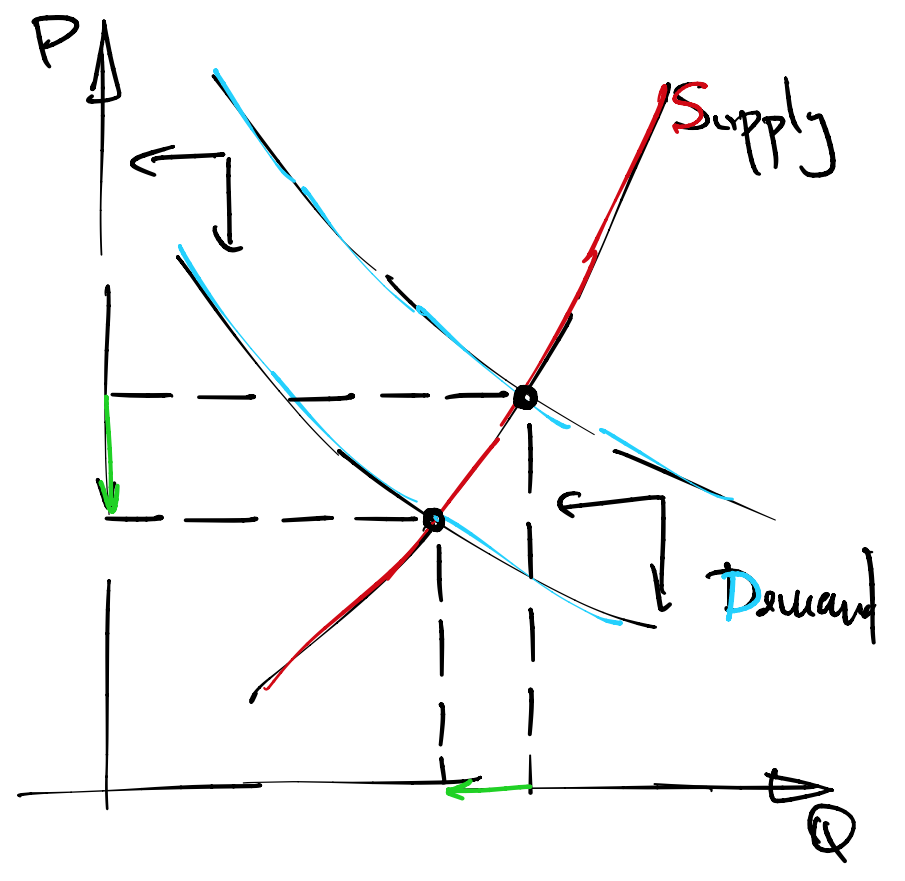
\includegraphics[width=.7 \textwidth]{dem_contract.png}
\end{figure}
\end{frame}

\begin{frame}{Появление субститутов}
И только в результате пересечения с предложением, мы можем утверждать о собственно падении (значения) спроса.

Формально замоделировать появление комплемента можно, например, при помощи полезности Кобб-Дугласа. Пусть для товара $x$ появился близкий субститут $\tilde x$ так, что полезность изменилась следующим образом.
$$ x^{1/2} \quad \to \quad x^{1/4}\tilde x^{1/4}$$
Проанализируйте, как изменится кривая спроса $x(p)$ как функция от собственной цены.

\end{frame}

\section{Появление комплементов}

\begin{frame}{Появление комплементов}

Когда появляется новый комплемент к нашему товару, то мы считаем, что спрос на него растет (расширяется). Представьте себе, что ученые открыли бы способ использовать старые покрышки вместо ядерного топлива. Это привело бы к увеличению спроса (даже на новые) покрышки и повышению цены.

\end{frame}

\begin{frame}{Появление комплементов}

Чуть сложнее смоделировать появление комплемента, но, при большом желании можно.
$$ x^{1/2} \quad \to \quad x^{1/2} + \min(x, \tilde x)$$

Тот же вопрос.

\end{frame}

\section{Изменение цен другие товары}

\begin{frame}{Изменение цен другие товары}

Когда цены другох товаров меняются, то сдвигается кривая спроса на наш товар, в зависимости от того, были ли они (валовыми) субститутами или комплементами.

Мы знаем, что Леонтьевская полезность дает комплементарную связь между товарами, а Кобб-Дуглас что то среднее между субститутом и комплементом, так как спрос там не реагирует на изменения цен других товаров. 
	
\end{frame}

\begin{frame}{Изменение цен другие товары}

Товары в CES полезности, которая рассмотрена во 2 лекции будут связаны как субституты. 

Действительно, вспомним формулу:
\begin{gather*}
x^{\ast} = \frac{\alpha^{\sigma} p^{1-\sigma}}{\alpha^{\sigma} p^{1-\sigma} + (1-\alpha)^{\sigma} q^{1-\sigma}}\frac{I}{p},\\
y^{\ast} = \frac{(1-\alpha)^{\sigma} q^{1-\sigma}}{\alpha^{\sigma} p^{1-\sigma} + (1-\alpha)^{\sigma} q^{1-\sigma}}\frac{I}{q}.
\end{gather*}
	
\end{frame}

\section{Изменение дохода и числа потребителей}

\begin{frame}{Изменение дохода и числа потребителей}

Довольно предсказуемо ведет себя кривая спроса при увеличении дохода - она будет расширяться. Конечно, если товар не нормальный, будет верно обратное, но мы уже знаем, что для этого нужны очень специфические условия.

При увеличении числа потребителей кривая спроса, конечно же, расширяется. Если потребителей стало больше, скажем, за счет, открытия новых рынков сбыта товара, то количество запрошенного товара увеличится при каждом уровне цены.

\end{frame}

\section{Изменение собственной цены}
\begin{frame}{Изменение дохода и числа потребителей}
Ну и, конечно, тяжело обойти стороной самое главное - изменение собственной цены.

Как обычно ведет себя кривая спроса при увеличении собственной цены?
\end{frame}

\section{Сдвиги кривых спроса (на факторы)}

\begin{frame}{Сдвиги кривых спроса (на факторы)}
Ничего не мешает нам исследовать частичное равновесие на рынке факторов производства. В таком случае, фирмы ведут себя как потребители. 

Поставщиками факторов могут являться другие фирмы, или может быть просто неизменная мировая цена на фактор, если речь идет о нефти, угле или металле.
	
\end{frame}

\begin{frame}{Сдвиги кривых спроса (на факторы)}

Вот список событий, которые могут спровоцировать сокращение спроса на факторы производства.

\begin{itemize}
\item общее улучшение технологии, скажем, за счет равномерного роста производственной функции
\item увеличение цены на фактор, который находится в комплиментарной связи (в смысле производства, подумайте  что это значит) с тем, который мы изучаем
\item уменьшение цены на фактор, который является субститутом (опять же, в смысле производства)
\item уменьшение цены на конечный товар, использующий этот фактор в производстве
\item уменьшение числа фирм (внезапное)
\end{itemize}
	
\end{frame}

\section{Сдвиги кривых предложения}
\begin{frame}{Сдвиги кривых предложения}


Зафиксируем кривую спроса $Q^d(P)$. Сдвиги кривых предложения чуть более хитрые, поскольку важны оси.

\begin{itemize}
\item сокращение кривой предложение это уменьшение Q...
\item расширение кривой предложение это увеличение Q...
\end{itemize}

... при том же P.

Поскольку цена, как правило, находится на вертикальной оси, то расширение это движение вправо. Постарайтесь не запутаться.
	
\end{frame}

\section{Увеличение цен на факторы}

\begin{frame}{Увеличение цен на факторы}
	
Довольно стандартной является ситуация, что цены на факторы производства растут. Напомню, что функция издержек зависит от цен на факторы. 

Как уровень производства зависит от цен на факторы?

Попробуйте ответить интуитивно.
\end{frame}

\begin{frame}{Увеличение цен на факторы}
	
Поскольку функция издержек это огибающая издержек, ее наклон по параметрам равен условному спросу на факторы производства, то есть, у нее положительный наклон:
$$ \nabla_p TC(p, y) = x^{\ast}(p, y) \geqslant 0$$
Но, на самом деле, этого еще не достаточно, чтобы заявить о монотонности оптимального уровня производства по ценам на факторы. 
\end{frame}

\begin{frame}{Увеличение цен на факторы}
	
Для этого надо вспомнить, что гессиан (вогнутой по $p$) функции издержек это градиент от условного спроса
$$ \nabla^2_p TC(p, y) = \nabla_p x^{\ast}(p, y) \leqslant 0.$$

A значит, сам условный спрос монотонно убывает по ценам. Ну а раз условный спрос убывает, то и количество произведенного товара, конечно же, тоже убывает.
	
\end{frame}

\begin{frame}{Увеличение цен на факторы}
\begin{figure}[hbt]
\centering
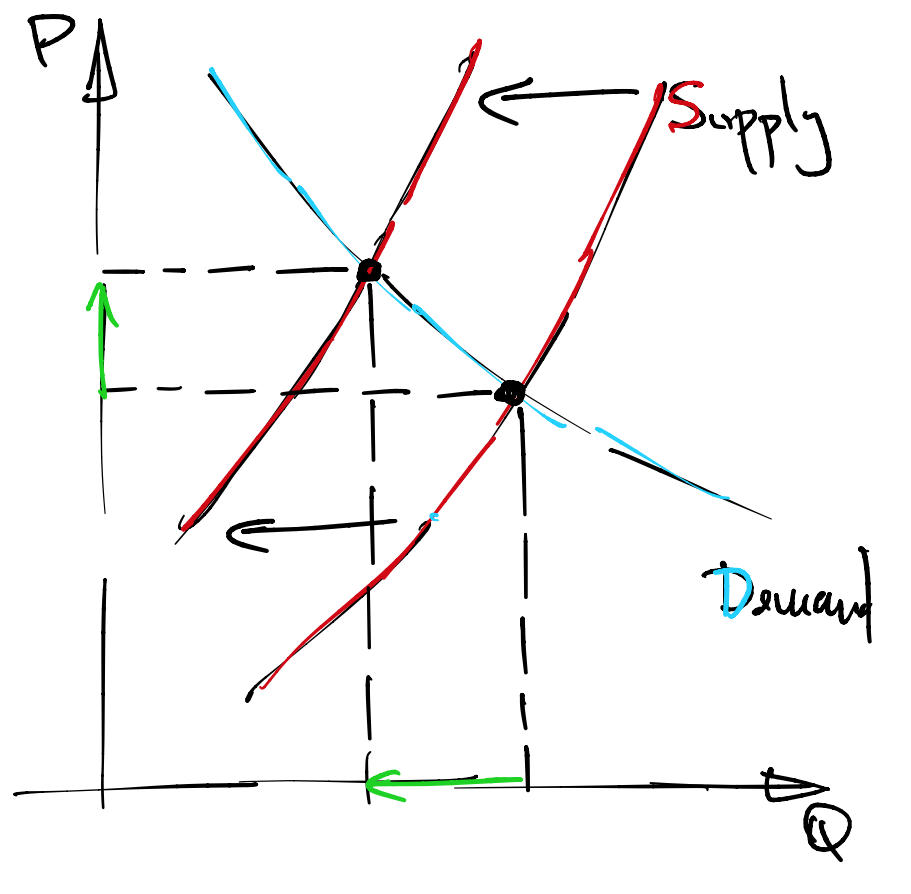
\includegraphics[width=.7 \textwidth]{sup_contract.png}
\end{figure}
\end{frame}

\section{Санкции, квоты, катаклизмы}
\begin{frame}

Конечно же, когда вмешивается некоторый внешний фактор, физически запрещающий производить определенный товар, то предложение этого товара должно упасть. Примерами могут служить
\begin{itemize}
\item запрет на оборот (вредного) товара
\item пожары, цунами...
\item войны, санкции...
\end{itemize}
\end{frame}


\section{Цена на сам товар}
\begin{frame}{Цена на сам товар}
Как ведет себя кривая предложения при увеличении цены на сам товар?
\end{frame}

\section{Агрегирование}
\begin{frame}{Агрегирование}
Иногда мы будем моделировать несколько потребителей и несколько производителей. Тогда, необходимо сложить их соответствующие кривые спроса и предложений "горизонтально". То есть необходимо сложить решения соответствующих задач потребителя/производителя, при каждой возможной цене.

В следующих примерах я буду использовать обозначение $p,q,r$ для цен товаров и факторов, a $Q^s_{\sum}$, $Q^d_{\sum}$ для агрегированного предложения и спроса на товар $x$.
\end{frame}

\section{Пример со спросом}
\begin{frame}{Пример со спросом}
Предположим, что есть два потребителя с одинаковым доходом, но разной полезностью:
$$ U_1(x,y) = \sqrt(x,y), \quad U_2(x,y) = \min(x,y)$$

Нас будет интересовать агрегированный спрос, например, на товар $х$, как функция от его цены $p$.
$$ Q^d_{\sum}(p) = \frac{I}{2p} + \frac{I}{p + q} $$

где $q$ это цена товара $y$, являющаяся параметром задачи.
	
\end{frame}

\section{Пример с предложением}

\begin{frame}{Пример с предложением}
Предположим, что есть два производителя с технологиями:
$G_1(x,y) = 2 x^2 + y^2 \leqslant z, \quad G_2(x,y) = x^2 + 2 y^2 \leqslant z$

где $z$ это единый фактор производства с ценой $r$.

\end{frame}

\begin{frame}{Пример с предложением}
Выпишем лагранжианы:
\begin{gather*}
\mathcal{L}_1 = px + qy - rz - \lambda(2x^2 + y^2 - z)\\
\mathcal{L}_2 = px + qy - rz - \gamma(x^2 + 2y^2 - z)
\end{gather*}

Отсюда легко находятся множители лагранжа $\lambda = \gamma = r$, и, собственно предложения товара $x$ от каждого из заводов.
$$Q^s_{\sum}(p) = \frac{p}{4 r} + \frac{p}{2r}.$$
\end{frame}

\section{Частичное равновесие}
\begin{frame}{Частичное равновесие}

\begin{definition}
\textbf{Частичным равновесием} на рынке товара $x$ называется цена $P^{\ast}$ и количество $Q^{\ast}$ лежащее в пересечении агрегированных кривых спроса и предложения.
$$(P^{\ast},Q^{\ast}) \in Q^d_{\sum}(p) \cap Q^s_{\sum}(p)$$
\end{definition}
	
\end{frame}

\begin{frame}{Частичное равновесие}

Как правило, частичное равновесие существует, поскольку кривые спроса монотонны и непрерывны по общим теоремам. Однако, есть исключения. 

Например, при анализе предложения в присутствие фиксированных издержек, фирма <<разрывно>> перемещает свое предложение в ноль, в момент, когда цена проходит через точку закрытия рынка. 

Это значит, что равновесия может не быть, см. иллюстрацию.
	
\end{frame}

\begin{frame}{Частичное равновесие}

\begin{figure}[hbt]
\centering
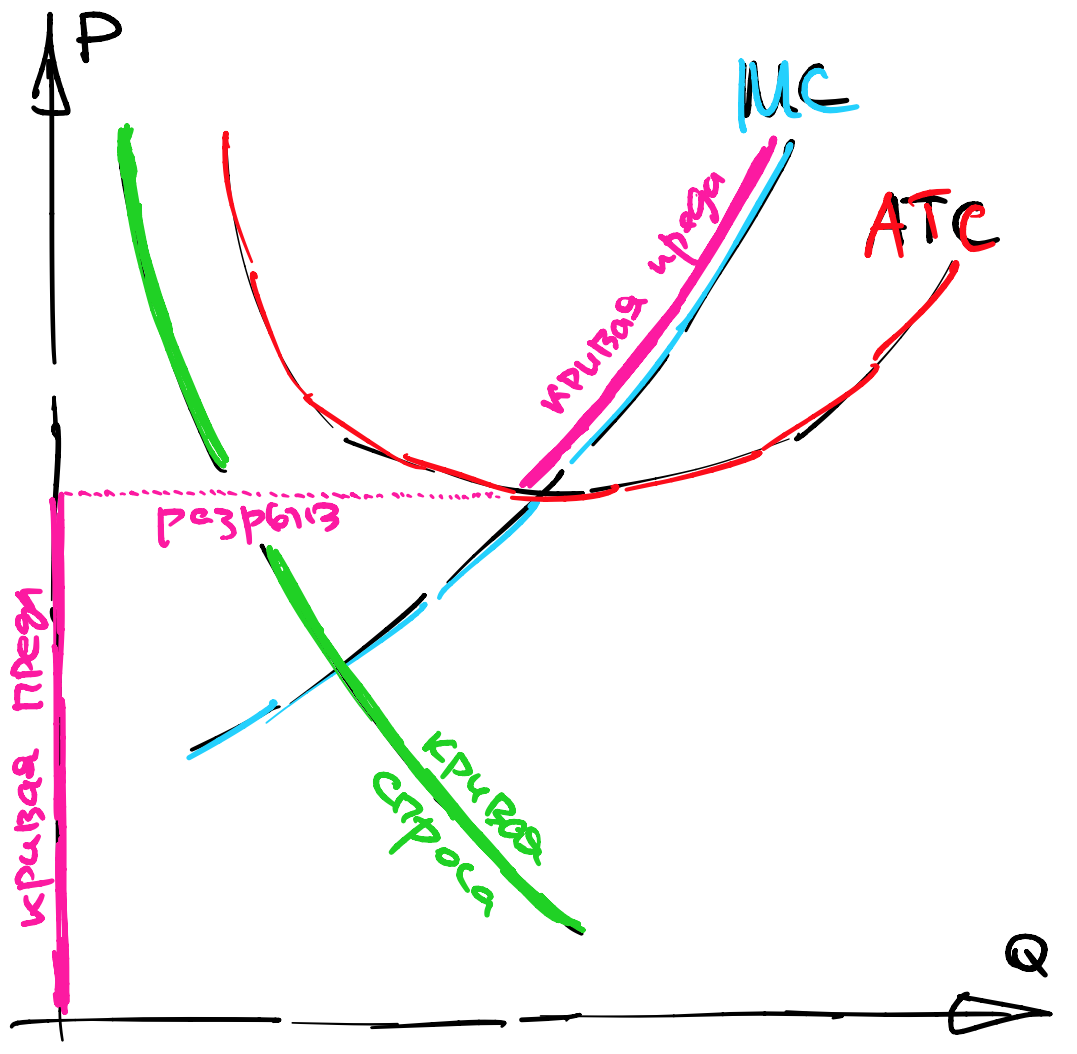
\includegraphics[width=.7 \textwidth]{nonexistence.png}
\end{figure}
	
\end{frame}

\begin{frame}{Частичное равновесие}

Так это что получается, невыпуклая задача?
	
\end{frame}

\begin{frame}{Частичное равновесие}

Да, потому что максимум в $\max(0, \pi)$ это выпуклое преобразование, а нам нужно, ну хотя бы вогнутое. 
	
\end{frame}

\section{Конец}

\end{document}